\documentclass{article}
\iffalse
This file is protected by Copyright. Please refer to the COPYRIGHT file
distributed with this source distribution.

This file is part of OpenCPI <http://www.opencpi.org>

OpenCPI is free software: you can redistribute it and/or modify it under the
terms of the GNU Lesser General Public License as published by the Free Software
Foundation, either version 3 of the License, or (at your option) any later
version.

OpenCPI is distributed in the hope that it will be useful, but WITHOUT ANY
WARRANTY; without even the implied warranty of MERCHANTABILITY or FITNESS FOR A
PARTICULAR PURPOSE. See the GNU Lesser General Public License for more details.

You should have received a copy of the GNU Lesser General Public License along
with this program. If not, see <http://www.gnu.org/licenses/>.
\fi

\author{} % Force author to be blank
%----------------------------------------------------------------------------------------
% Paper size, orientation and margins
%----------------------------------------------------------------------------------------
\usepackage{geometry}
\geometry{
	letterpaper,			% paper type
	portrait,				% text direction
	left=.75in,				% left margin
	top=.75in,				% top margin
	right=.75in,			% right margin
	bottom=.75in			% bottom margin
 }
%----------------------------------------------------------------------------------------
% Header/Footer
%----------------------------------------------------------------------------------------
\usepackage{fancyhdr} \pagestyle{fancy} % required for fancy headers
\renewcommand{\headrulewidth}{0.5pt}
\renewcommand{\footrulewidth}{0.5pt}
\rhead{\small{ANGRYVIPER Team}}
%----------------------------------------------------------------------------------------
% Appendix packages
%----------------------------------------------------------------------------------------
\usepackage[toc,page]{appendix}
%----------------------------------------------------------------------------------------
% Defined Commands & Renamed Commands
%----------------------------------------------------------------------------------------
\renewcommand{\contentsname}{Table of Contents}
\renewcommand{\listfigurename}{List of Figures}
\renewcommand{\listtablename}{List of Tables}
\newcommand{\todo}[1]{\textcolor{red}{TODO: #1}\PackageWarning{TODO:}{#1}} % To do notes
\newcommand{\code}[1]{\texttt{#1}} % For inline code snippet or command line
%----------------------------------------------------------------------------------------
% Various pacakges
%----------------------------------------------------------------------------------------
\usepackage{hyperref} % for linking urls and lists
\usepackage{graphicx} % for including pictures by file
\usepackage{listings} % for coding language styles
\usepackage{rotating} % for sideways table
\usepackage{pifont}   % for sideways table
\usepackage{pdflscape} % for landscape view
%----------------------------------------------------------------------------------------
% Table packages
%----------------------------------------------------------------------------------------
\usepackage{longtable} % for long possibly multi-page tables
\usepackage{tabularx} % c=center,l=left,r=right,X=fill
\usepackage{float}
\floatstyle{plaintop}
\usepackage[tableposition=top]{caption}
\newcolumntype{P}[1]{>{\centering\arraybackslash}p{#1}}
\newcolumntype{M}[1]{>{\centering\arraybackslash}m{#1}}
%----------------------------------------------------------------------------------------
% Block Diagram / FSM Drawings
%----------------------------------------------------------------------------------------
\usepackage{tikz}
\usetikzlibrary{shapes,arrows,fit,positioning}
\usetikzlibrary{automata} % used for the fsm
%----------------------------------------------------------------------------------------
% Colors Used
%----------------------------------------------------------------------------------------
\usepackage{colortbl}
\definecolor{blue}{rgb}{.7,.8,.9}
\definecolor{ceruleanblue}{rgb}{0.16, 0.32, 0.75}
\definecolor{drkgreen}{rgb}{0,0.6,0}
\definecolor{deepmagenta}{rgb}{0.8, 0.0, 0.8}
\definecolor{cyan}{rgb}{0.0,0.6,0.6}
\definecolor{maroon}{rgb}{0.5,0,0}
%----------------------------------------------------------------------------------------
% Update the docTitle and docVersion per document
%----------------------------------------------------------------------------------------
\def\docTitle{Component Data Sheet}
\def\docVersion{1.4}
%----------------------------------------------------------------------------------------
\date{Version \docVersion} % Force date to be blank and override date with version
\title{\docTitle}
\lhead{\small{\docTitle}}

\def\comp{timestamper}
\edef\ecomp{timestamper}
\def\Comp{Timestamper}
\graphicspath{ {figures/} }

\begin{document}

\section*{Summary - \Comp}
\begin{tabular}{|c|M{13.5cm}|}
	\hline
	\rowcolor{blue}
	                  &                        \\
	\hline
	Name              & \comp                  \\
	\hline
	Worker Type       & Application            \\
	\hline
	Version           & v\docVersion \\
	\hline
	Release Date      & September 2018 \\
	\hline
	Component Library & ocpi.assets.util\_comps \\
	\hline
	Workers           & \comp.hdl              \\
	\hline
	Tested Platforms  & xsim, isim, modelsim, Matchstiq-Z1(PL) \\
	\hline
\end{tabular}

\section*{Functionality}
\begin{flushleft}
	The Timestamper component inputs complex IQ data and outputs complex IQ data prepended with a timestamp. One timestamp is sent for each data message produced on the output.
\end{flushleft}

\section*{Worker Implementation Details}
\subsection*{\comp.hdl}
\begin{flushleft}
	A timing diagram of the output interface for this component can be seen in Figure \ref{fig:timestamper_timing_diagram}.\par\bigskip
	\noindent Timestamps are provided as an input to the component on the time interface. The timestamp is a 64 bit number with the first 32 bits corresponding to seconds and the last 32 bits corresponding to fractional seconds. When a valid message is detected on the input, the timestamp is registered by the component and given on the output interface. Timestamps and data are given on the output interface using different opcodes.\par\bigskip
	The time interface from which the timestamps are generated originates from the OpenCPI time server, which is instanced as part of the platform worker. Furthermore, an additional component (time client) is dynamically instanced by the framework for all components which declare time interfaces. The time client communicates with the time server and produces the time interface seen by the component.
\end{flushleft}
\begin{figure}[p]
	\centering
	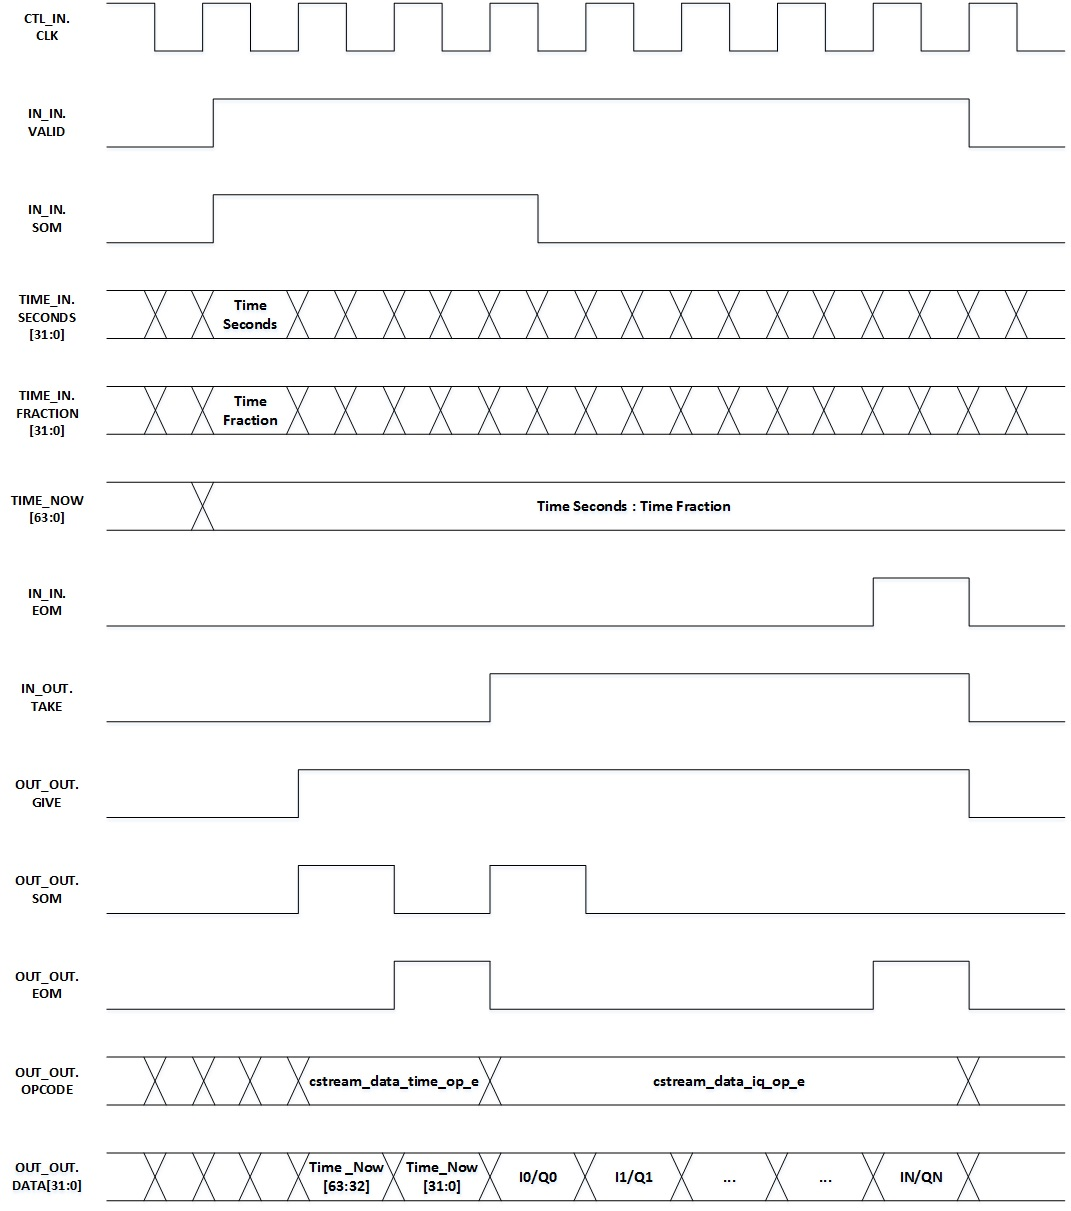
\includegraphics[scale=0.6]{timestamper_timing_diagram}
	\caption{Timestamper Output Timing Diagram}
	\label{fig:timestamper_timing_diagram}
\end{figure}
\pagebreak

\section*{Block Diagrams}
\subsection*{Top level}
\begin{center}
	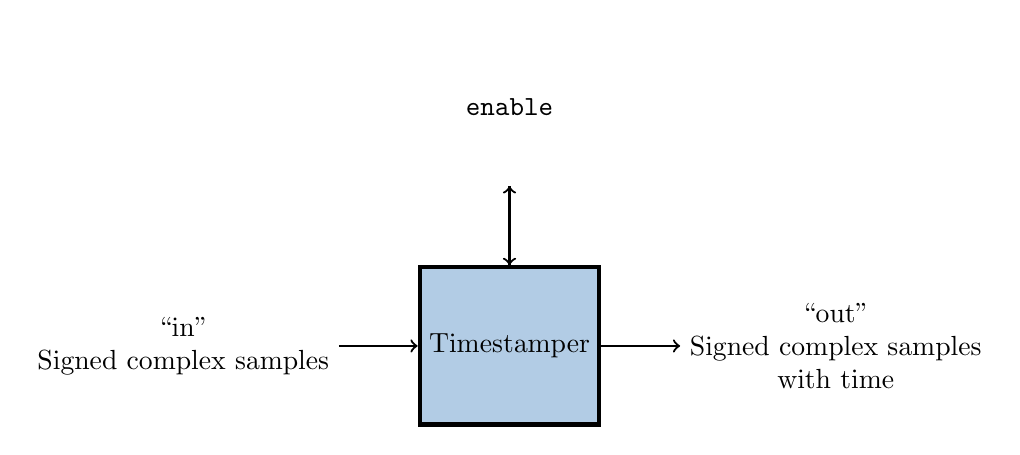
\begin{tikzpicture}[% List of styles applied to all, to override specify on a case-by-case
			every node/.style={
				align=center,  		% use this so that the "\\" for line break works
				minimum size=2cm	% creates space above and below text in rectangle
			},
			every edge/.style={draw,thick}
		]
		\node[rectangle,ultra thick,draw=black,fill=blue](R2){\Comp};
		\node[rectangle,draw=white,fill=white](R3)[left= of R2]{``in'' \\ Signed complex samples};
		\node[rectangle,draw=white,fill=white](R4)[right= of R2]{``out'' \\ Signed complex samples\\ with time};
		\node[rectangle,draw=white,fill=white](R5)[above= of R2]{\verb+enable+};
		\path[->]
		(R3)edge []	node [] {} (R2)
		(R2)edge []	node [] {} (R4)
		(R2)edge []	node [] {} (R5)
		(R5)edge []	node [] {} (R2)
		;
	\end{tikzpicture}
\end{center}

\section*{Source Dependencies}
\subsection*{\comp.hdl}
\begin{itemize}
	\item projects/assets/components/util\_comps/\comp.hdl/\comp.vhd
\end{itemize}

\begin{landscape}
	\section*{Component Spec Properties}
	\begin{scriptsize}
		\begin{tabular}{|p{3cm}|p{1.5cm}|c|c|c|p{1.5cm}|p{1cm}|p{7cm}|}
			\hline
			\rowcolor{blue}
			Name          & Type & SequenceLength & ArrayDimensions & Accessibility      & Valid Range & Default & Usage                        \\
			\hline
			\verb+enable+ & Bool & -              & -               & Writable, Readable & Standard    & true    & Enable or bypass timestamper \\
			\hline
		\end{tabular}
	\end{scriptsize}

	\section*{Worker Properties}
	There are no worker implementation-specific properties for this component

	\section*{Component Ports}
	\begin{scriptsize}
		\begin{tabular}{|M{2cm}|M{1.5cm}|M{4cm}|c|c|M{9cm}|}
			\hline
			\rowcolor{blue}
			Name & Producer & Protocol                       & Optional & Advanced & Usage                                  \\
			\hline
			in   & false    & iqstream\_protocol             & false    & -        & Signed complex samples                 \\
			\hline
			out  & true     & iqstream\_protocol\_with\_sync & false    & -        & Signed complex samples with timestamps \\
			\hline
		\end{tabular}
	\end{scriptsize}
	\section*{Worker Interfaces}
	\subsection*{\comp.hdl}
	\begin{scriptsize}
		\begin{tabular}{|M{2cm}|M{1.5cm}|c|c|M{12cm}|}
			\hline
			\rowcolor{blue}
			Type            & Name & DataWidth & Advanced                         & Usage                                    \\
			\hline
			StreamInterface & in   & 32        & numberOfOpcodes=256              & Signed complex samples                   \\
			\hline
			StreamInterface & out  & 32        & numberOfOpcodes=256              & Signed complex samples with timestamps   \\
			\hline
			TimeInterface   & time & -         & SecondsWidth=32 FractionWidth=32 & Time interface provided from Time Server \\
			\hline
		\end{tabular}
	\end{scriptsize}
\end{landscape}

\section*{Control Timing and Signals}
\begin{flushleft}
	The Timestamper HDL worker uses the clock from the Control Plane and standard Control Plane signals.\\
	\begin{tabular}{|M{4.5cm}|M{1cm}|M{1cm}|M{1.5cm}|M{2cm}|M{1cm}|M{1cm}|M{2.5cm}|}
		\hline
		\rowcolor{blue}
		Latency         \\
		\hline
		3               \\
		\hline
	\end{tabular}\par\bigskip
	\noindent Data presented on the input appears on the output 3 clock cycles later. 2 of the 3 clock cycles consist of a time message
\end{flushleft}

\begin{landscape}
\section*{Worker Configuration Parameters}
\subsubsection*{\comp.hdl}
\input{../../\ecomp.hdl/configurations.inc}
\section*{Performance and Resource Utilization}
\subsubsection*{\comp.hdl}
\input{../../\ecomp.hdl/utilization.inc}
\end{landscape}
\section*{Test and Verification}
\begin{flushleft}
	Two test cases are implemented to validate the \Comp{} component:
	\begin{itemize}
		\item[1)] Bypass mode
		\item[2)] Normal mode
	\end{itemize}
	For both cases, the input file is a series of 8 ramps with 32-bit values ranging from 0 to 512.\par\medskip
	For case 1, the input data is forwarded to the output port. For verification, the output file is byte-wise compared to the input file.\par\medskip
	For case 2,  the expected output waveform is the identical ramp with timestamps inserted before each data message. For verification, the timestamps are extracted and checked for incrementing values
\end{flushleft}
\end{document}
